\documentclass[wide,a4paper,titlepage,12pt] {article}
\usepackage{polski}
\usepackage[utf8]{inputenc}
\usepackage{listings}
\usepackage{float}
\usepackage{slashbox}
\usepackage[table]{xcolor}
\usepackage{graphicx,pdflscape}
\usepackage{placeins}


\title{Grafika komputerowa}
\author{Tymon Tobolski (181037)}

% Title page layout (fold)
\makeatletter
\renewcommand{\maketitle}{
\begin{titlepage}
  \begin{center}
    \vspace*{3cm}
    \LARGE \@title \par
    \vspace{2cm}
    \textit{\small Autor:}\par
    \normalsize \@author\par \normalsize
    \vspace{3cm}
    \textit{\small Prowadzący:}\par
    Dr inż. Tomasz Kapłon \par
    \vspace{2cm}
    Wydział Elektroniki\\ III rok\\ Pn TP 08.15 - 11.00\par
    \vspace{4cm}
    \small 14 listopada 2011
  \end{center}
\end{titlepage}
}
\makeatother
  \lstset{
    language=c++,
    basicstyle=\ttfamily\scriptsize,
    numbers=left,
    numberstyle=\scriptsize,
    stepnumber=10,
    numbersep=9pt,
    showspaces=false,
    showstringspaces=false,
    showtabs=false,
    breaklines=true,
  }

\begin{document}
\maketitle
  \section{Cel laboratorium}
  \paragraph{}
  Celem laboratorium było zaprezentowanie możliwości oświetlania obiektów scen 3-D przy użyciu biblioteki OpenGL.

  \section{Wprowadzenie źródła światła}
  \paragraph{}
  Pierwsze zadanie polegało na wyświetleniu białego czajnika oświetlonego za pomocą jednego źródła światła.
  \paragraph{}
  \lstinputlisting{1.cpp}

  \begin{figure}[h!]
    \begin{center}
      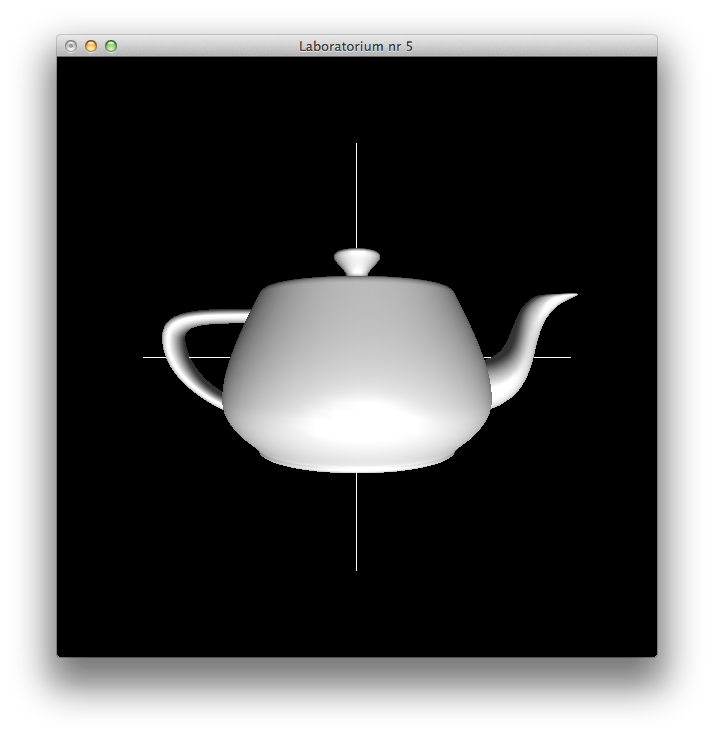
\includegraphics[width=\textwidth]{1.png}
      \caption{Czajnik oświetlony jednym źródłem światła}
    \end{center}
  \end{figure}


  \section{Wprowadzenie drugiego źródła światła}
  \paragraph{}
  Drugie zadanie polegało na wprowadzenie kolejnego żródła światła o innym kolorze i oświetlenie modelu jajka oraz dodaniu możliwości sterowania położeniem źródeł światła za pomocą myszki.
  \paragraph{}
  \lstinputlisting{2.cpp}

  \begin{figure}[h!]
    \begin{center}
      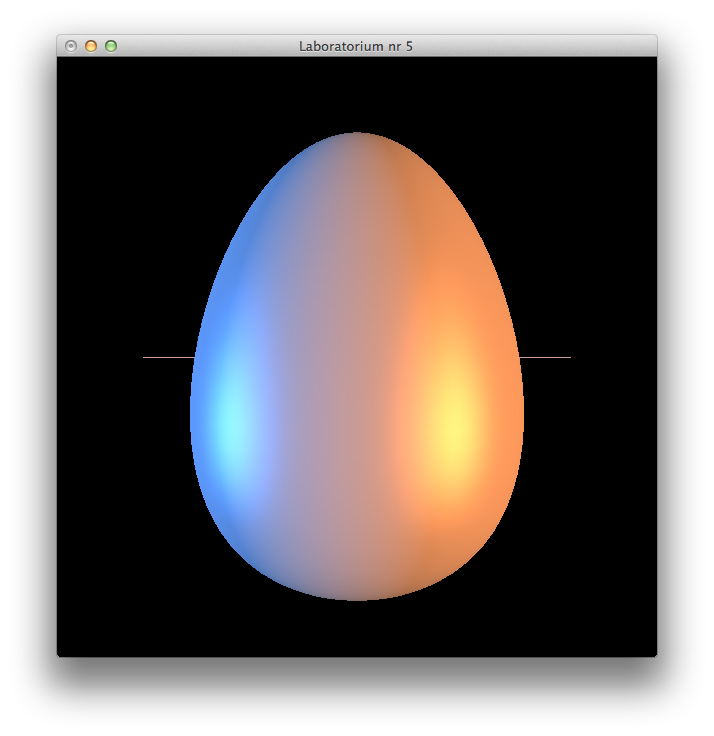
\includegraphics[width=\textwidth]{2.png}
      \caption{Jajko oświetlone dwoma źródłami światła}
    \end{center}
  \end{figure}

  \newpage
  \section{Wnioski}
  \paragraph{}
  Dodanie źródła światła do sceny 3-D przy wykorzystaniu biblioteki OpenGL jest stosunkowo prostym zadaniem. Największym problemem podczas realizacji laboratorium okazało się wyliczenie wektorów normalnych do powierzchni jajka.

\end{document}